\documentclass{beamer}

\usepackage[czech, english]{babel}
\usepackage[utf8]{inputenc}	
\usepackage[square,sort,comma,numbers]{natbib}
\usepackage{textpos}
\usepackage{listings}

\usetheme{Boadilla}
\title{MMDOS \\ Síťové analýzy PID}
\author{Michael Kala a Petra Millarová}
\date{únor 2019}

\begin{document}

\begin{frame}
\titlepage
\end{frame}

\begin{frame}
\section{Úvod}
\frametitle{Zadání}
\begin{block}{}
 \textit{Konzolová aplikace, která provádí síťové analýzy nad daty PID za využití pgRouting extenze PostGISu} 
 \end{block}
 
\begin{itemize}
	\item vstup - adresy počátečního a koncového bodu
	\item výstup - nejkratší cesta MHD spolu s doporučenými přestupy
\end{itemize}
\end{frame}

\begin{frame}
\section{Data}
\frametitle{Zdroje dat}
\begin{itemize}
	\item Adresní místa RÚIAN Hlavního města Prahy - nahlížení do KN - formát *.csv
	\item Trasy linek PID - portál opendata Hlavního města Prahy - formát *.shp
	\item Zastávky PID - portál opendata Hlavního města Prahy - formát *.shp
\end{itemize}
\end{frame}


\begin{frame}
\frametitle{Zpracování dat}
\begin{itemize}
	\item tvroba tabulky a geometrie pro adresní místa
	\item převod dat PID ze *.shp do tabulek
	\item odstranění nočních linek z dat PID
	\item přetypování sloupce zast\_uzel
\end{itemize}
\end{frame}

\begin{frame}[fragile]
\section{Topologie}
\frametitle{Topologie - hrany}	
\begin{itemize}
	\item přiřazení správných zast\_uzel do sloupců source a target pomocí skriptu
\end{itemize}
\begin{exampleblock}{}
\begin{lstlisting}[language=sql]
SELECT DISTINCT ON(t.gid) t.gid, z.zast_uzel_ 
FROM trasy t, zastavky z 
WHERE ST_DWithin(ST_StartPoint(ST_LineMerge(t.geom)), z.geom, 500) 
AND t.zast_id_od = z.zast_id
\end{lstlisting}
\end{exampleblock}

\end{frame}

\begin{frame}[fragile]
\frametitle{Topologie - uzly}	

\begin{itemize}
	\item vytvoření tabulky uzlů pomocí funkce pgr\_createVerticesTable a přejmenování sloupce \texttt{the\_geom} na \texttt{geom}
\end{itemize}

\begin{exampleblock}{}
\begin{lstlisting}[language=sql]
SELECT pgr_createVerticesTable('trasy','geom','source','target');
ALTER TABLE trasy_vertices_pgr rename column the_geom to geom;
\end{lstlisting}
\end{exampleblock}

\end{frame}

\begin{frame}[fragile]
\section{Konzolová aplikace}
\frametitle{Konzolová aplikace - pomocné SQL funkce}
\begin{exampleblock}{}
\begin{lstlisting}[language=sql]
FindStationName(id INTEGER)
FindVertexID(cd INTEGER, co INTEGER, u VARCHAR)
FindVertexIDcd(cd INTEGER, u VARCHAR)
FindVertexIDori(co INTEGER, u VARCHAR)
FindVertexIDst(u VARCHAR)
\end{lstlisting}
\end{exampleblock}
\end{frame}

\begin{frame}[fragile]
\frametitle{Konzolová aplikace - výpočet nejkratší trasy}
\begin{exampleblock}{}
\begin{lstlisting}[language=sql]
SELECT z.zast_nazev, trasy.l_metro, trasy.l_tram, trasy.l_bus, trasy.l_lan, trasy.l_vlak, trasy.l_lod, node
FROM pgr_dijkstra('SELECT gid as id, source, target, CAST(shape_leng as REAL) as cost FROM trasy', id_from, id_to) 
JOIN (SELECT DISTINCT(zastavky.zast_uzel_), zastavky.zast_nazev FROM zastavky) AS z ON node = z.zast_uzel_ L
EFT JOIN trasy ON edge = trasy.gid ORDER BY seq;"
\end{lstlisting}
\end{exampleblock}
\end{frame}

\begin{frame}
\frametitle{Konzolová aplikace - výpis zastávek}
\begin{itemize}
	\item \texttt{trasy} - v každém úseku údaje o všech linkách, které tudy vedou
	\item průchod nejkratší trasou a výběr linek s nejmenším počtem přestupů: 
	\begin{enumerate}
		\item průchod všech linek projíždějících první zastávkou, výpočet dosahu každé linky
	\item přiřazení čísla linky s nejdelším dosahem
	\item zpakování kroků 1 a 2
	\end{enumerate}
\end{itemize}
\end{frame}

\begin{frame}
\frametitle{Konzolová aplikace - ukázka výstupu}

\begin{figure}[h]
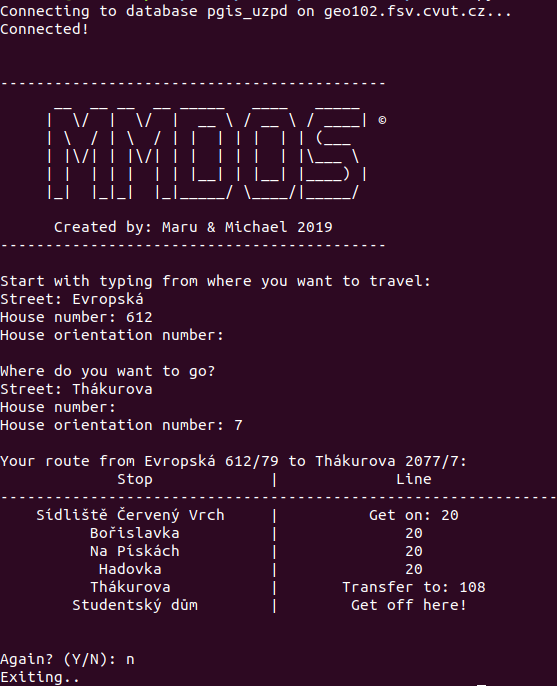
\includegraphics[scale=0.35]{ukazka.png}
\end{figure}
\end{frame}






\begin{frame}
\section{Závěr}
%\begin{columns}
%
%\column{0.45\textwidth}
%
%\column{0.55\textwidth}
%
%\end{columns}
\frametitle{Závěr - problémy a jejich řešení}
\begin{itemize}
	\item stejné "unikátní" ID v tabulce \texttt{zastavky}
	\item kombinace nočních a denních spojů
	\item ocenění tras - v reálu je trasa s méně přestupy rychlejší, než nejkratší trasa s více přestupy
\end{itemize}
\end{frame}

\begin{frame}
\Huge{\centerline{Děkujeme za pozornost.}}


\end{frame}
\end{document}